\documentclass{report}

\usepackage[utf8]{inputenc} % For input encoding
\usepackage{amsmath}        % For mathematical formulas
\usepackage{graphicx}       % For including images
\usepackage{geometry}       % For page layout
\usepackage{float}
\usepackage{hyperref}      % For hyperlinks
\geometry{a4paper, margin=1in}

\title{A study place and a friendly penguin}
\author{\textbf{Owlgorithm} \\ Pinar Erbil, Angela Remolina, Duvan Diaz, and Camilo Sinning}
\date{\today}

\begin{document}

\maketitle

% \tableofcontents % Optional: adds a table of contents
\newpage

\begin{abstract}
In this report, we present our proposal developed for the Education track at the GDG hackathon. Our project, titled \textit{A Study Place and a Friendly Penguin}, envisions a comprehensive and interactive study environment powered by agentic AI. At the core of our concept is a virtual penguin assistant designed to guide and support students throughout their learning journey. This AI-driven agent interacts with users, provides personalized feedback, and adapts to individual study habits to maximize learning outcomes, creates questions based on the subject and can control the widgets in the application. By integrating features such as study planning, content organization, reminders, and gamified interactions within a single application, we aim to improve how students engage with their educational materials. Our approach emphasizes engagement, adaptability, and the use of intelligent agents to foster effective learning experiences.
\end{abstract}

\chapter{Introduction}

This is a report to describe our ideas about the Education track in the GDG hackaton.

\section{Current State}

In this track, we are responsible for improving the Braynr application. The current state of the Braynr app is a desktop application that allows users to study and learn with the help of AI. The app is mainly focused on helping the students read and understand the content of their courses. The app has some features like flashcards, diagrams and AI-help. The app is designed to be used by students who want to learn and study in a more efficient way. The app is not very interactive and does not have a clear guide for the students. We are hoping to improve this app to make it more easy to interact with and more engaging for students.

\section{Proposed Challenge}
We needed to reimagine the app, trying to reinvent the way students learn and study. We wanted to create a more interactive and engaging experience for the users. The most important thing we needed to take into account was the use of agentic AI, which is a type of AI that can act on its own and make decisions based on the data it receives.

\section{Proposed Solution}

Our proposal consists of creating an entire environment for studying. We wanted the students to feel that they only have to open an single app where they can do everything. We wanted to create a space where the student can study, play, and have fun without any distractions. 

The central piece of our proposal is a friendly penguin, Pingu, that will be the guide of the student. Pingu will be the one who will help the student to study and learn. When the student interacts with the Pingu, it will be able to give feedback on their progress, answer their questions and quiz them. Furthermore, the penguin will be aware of the environment (date, time) and learn from the student. The main goal of this penguin agent is getting the student to learn and study. So, with the time it should learn the habits and methods that make the student the most productive such as the preferred pomodoro timer or the music the student prefers to listen.

Pingu will be on the screen all the time and will be able to interact with the user about what is on the screen. Furthermore, the penguin will be able to interact with all the available features, such as the calendar, the notes, the reminders, and the study planner, and help the student to use them in a more efficient way.

\footnotetext{Penguin animation credits: \url{https://giphy.com/pudgypenguins}}


\subsubsection{User Interface}

The figure~\ref{fig:ui} shows the landing page of the Braynr app.

\begin{figure}[H]
    \centering
    \begin{minipage}{0.48\textwidth}
        \centering
        
\includegraphics[width=\textwidth]{images/Home.png}
        \caption{Landing of the Braynr app}
        \label{fig:ui}
    \end{minipage}\hfill % \hfill fills the horizontal space
    \begin{minipage}{0.48\textwidth}
        \centering
        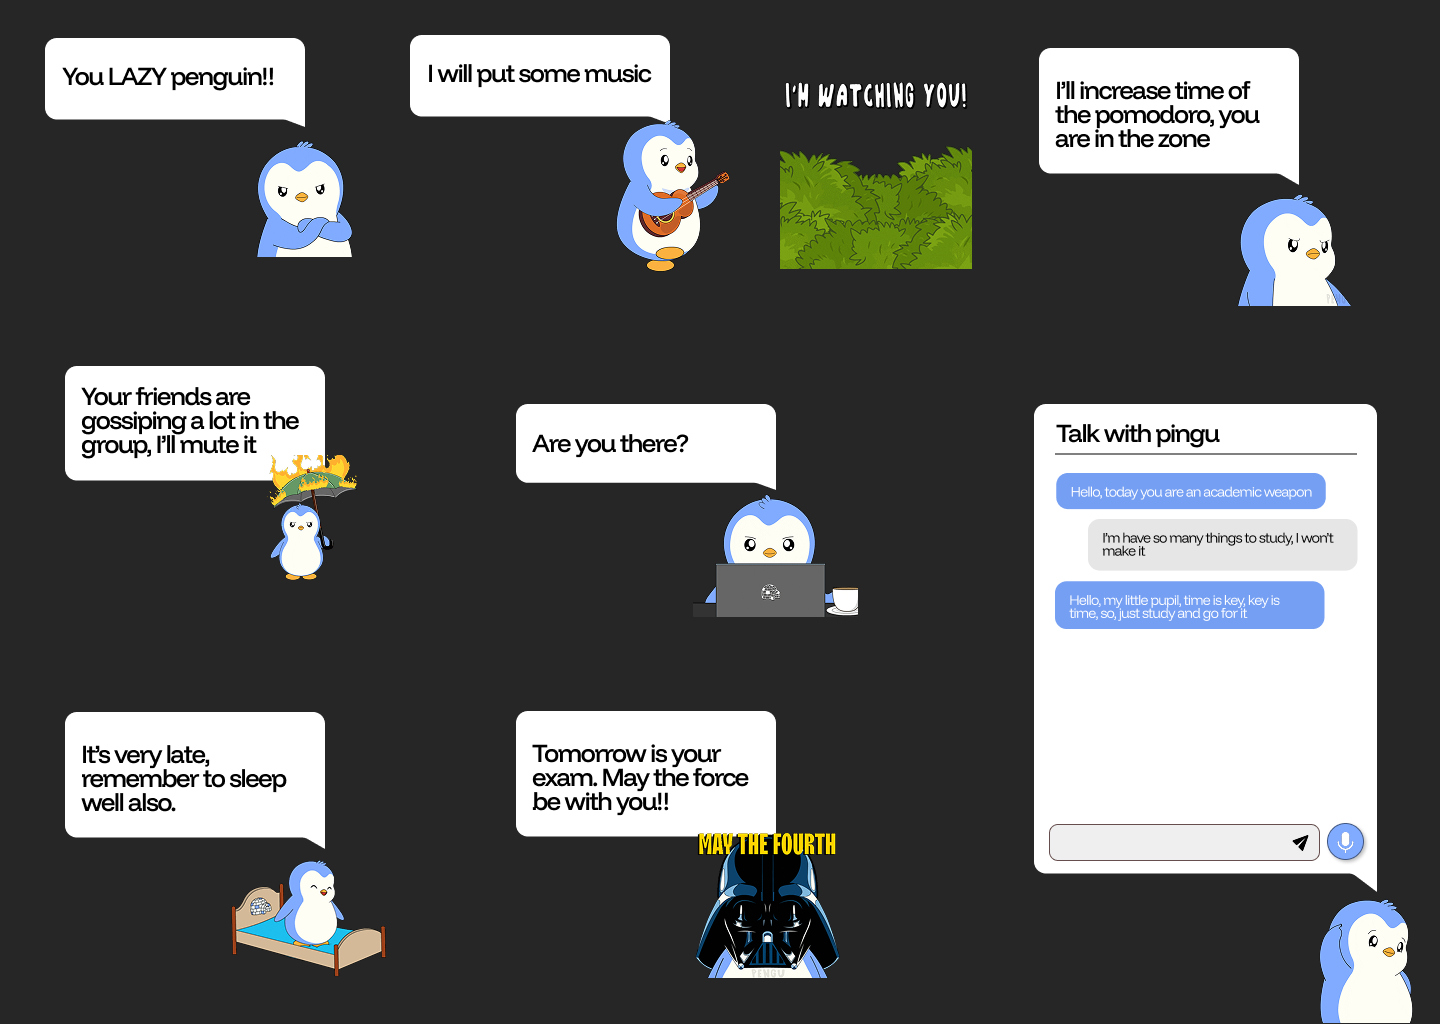
\includegraphics[width=\textwidth]{images/Pingu showcase.png}
        \caption{Penguin interacting with the user}
        \label{fig:chat}
    \end{minipage}
\end{figure}

Here are some examples of the penguin interacting with the user:

\section{Final Thoughts and Technical Details}
We think that this proposal is a good way to create a more interactive and engaging experience for the students. Pingu will be the perfect guide for the students, and it will help them to learn and study in a more efficient way. Our personalized penguin will work like a Reinforcement learner with a clear utility maximization (User learning).

How then, do we define a utility function with something as abstract as learning? Our little penguin will spontaneously ask the student questions about the content of the course, and based on the answers it will be able to have a rough idea about how much the user had learned. The penguin will also be able to ask the user about their preferences and habits, and based on that it will be able to create a personalized study plan for the student.

We are very excited about this proposal and we hope that you like it too.


\end{document}